% \documentclass[12pt,a4paper,titlepage]{article}
% \usepackage[utf8]{inputenc}
% \usepackage{polski}
% \usepackage{graphicx}
% \usepackage{tikz}
% \usepackage{pgfplots}
% \usepackage{pgfgantt}
% \usepackage{xcolor}
% \usepackage{floatrow}
% \usepackage{minted}
% \usepackage{times}
% \usepackage{tikz}
% \usepackage{pgfgantt}
% \usepackage{rotating}
% \usepackage{tikz-uml}
% \usepackage{hyperref}
% \usepackage{tabto}
% \tikzset{singlestate/.style={
%             draw,
%             fill=green!30, 
%             rounded corners, 
%             text width=4.5cm, 
%             align=center
%             }}
% \usetikzlibrary{matrix}
\documentclass[12pt,a4paper,titlepage]{article}
\usepackage[utf8]{inputenc}
\usepackage{polski}
\usepackage{graphicx}
\usepackage{tikz}
\usepackage{pgfplots}
\usepackage{pgfgantt}
\usepackage{xcolor}
\usepackage{floatrow}
\usepackage{minted}
\usepackage{amsmath}
\usepackage{caption}
\usepackage{url}
\usepackage{pgfgantt}
\usepackage{rotating}
\usepackage{tikz-uml}
\usepackage{hyperref}
\usepackage{tabto}
\usepackage{amssymb}

\tikzset{singlestate/.style={
            draw,
            fill=green!30, 
            rounded corners, 
            text width=4.5cm, 
            align=center
            }}
\usetikzlibrary{matrix}
\pgfplotsset{compat=1.16}
 
\setminted{
    linenos=true,
    autogobble,
    breaklines,
    frame=lines,
    framerule=1pt,
    framesep=10pt,
    fontsize=\small
}

\makeatletter

\newcommand{\texta}{Pomocne\\ \tiny (w osiągnięciu celu)\par}
\newcommand{\textb}{Szkodliwe\\ \tiny (w osiągnięciu celu)\par}
\newcommand{\textcn}{Pochodzenie wewnętrzne\\ \tiny (atrybuty produktu\slash firmy)\par}
\newcommand{\textdn}{Pochodzenie zewnętrzne\\ \tiny (atrybuty środowiska\slash rynku)\par}

\newcommand{\linia}{\rule{\linewidth}{0.4mm}}

\newcommand{\specialcell}[2][c]{
  \begin{tabular}[#1]{@{}c@{}}#2\end{tabular}
}

\renewcommand\listoflistingscaption{Spis listingów}

\renewcommand{\maketitle}{\begin{titlepage}
    \vspace*{1cm}
    \begin{center}\small
    Politechnika Wrocławska\\
    Wydział Elektroniki\\
    Internetowe Bazy Danych
    \end{center}
    \vspace{3cm}
    \noindent\linia
    \begin{center}
      \LARGE \textsc{\@title}
         \end{center}
     \linia
    \vspace{0.5cm}
    \begin{flushright}
    \begin{minipage}{7cm}
    \textit{\small Autor:}\\
    \normalsize \textsc{\@author} \par
    \end{minipage}
    \vspace{5cm}

     {\small Poniedziałek, 9\textsuperscript{15}-12\textsuperscript{00} TP}\\
        Dr inż. Roman Ptak
     \end{flushright}
    \vspace*{\stretch{6}}
    \begin{center}
    \@date
    \end{center}
  \end{titlepage}%
}
\makeatother
\author{Daniel Szewczyk, 226038\\
        Justyna Skalska, 225942}
\title{Projekt\\
\large(Sklep internetowy)}

\begin{document}
\maketitle
\newpage
\tableofcontents
\newpage
\listoffigures

\newpage
\listoflistings


\newpage

\section{Wstęp}
Głównym celem projektu jest zaprojektowanie oraz stworzenie witryny, dzięki której użytkownik będzie w stanie uzyskać dostęp do bazy danych z poziomu przeglądarki internetowej. Serwis ten będzie prostym sklepem internetowym pozwalającym na zakup różnego rodzaju deskorolek. Aby udało nam się wykonać projekt przed upływem wymaganych terminów zdecydowaliśmy się na wybór konkretnego produktu, który będzie posiadał szczególne dla siebie atrybuty.

Użytkownicy będą mieć przypisane funkcje, które pełnią na stronie. Może to być zwykły użytkownik witryny lub admin, który będzie miał dostęp do specjalnego panelu. Dzięki niemu będzie mógł przeglądać wszystkie dane zapisane w bazie sklepu, a także modyfikować część z nich, np. użytkowników, produkty oraz kategorie. Zwykły użytkownik będzie mógł przeglądać listę produktów, a także strony pojedynczego towaru, gdzie wypisane będą jego atrybuty. Każdy produkt będzie mógł być dodany do koszyka. Lista towarów wcześniej dodanych będzie dostępna na stronie koszyka, z której będzie można złożyć zamówienie.

Dostępna będzie także podstawowa wersja przeszukiwania katalogu przez podanie kodu produktu lub jego nazwy.

\newpage
\section{Technologie}
\label{sec:tech}
Przy pracy nad projektem wykorzystamy podane technologie:
\begin{itemize}
    \item Java (OpenJDK 13) \tab\url{https://jdk.java.net/13}
    \item Spring 5.2 \tab\url{https://spring.io}
    \item Spring Boot 2.2 \tab\url{https://spring.io/projects/spring-boot}
    \item Hibernate 5 \tab\url{https://hibernate.org}
    \item Lombok \tab\url{https://projectlombok.org/}
    \item Thymeleaf 3 \tab\url{https://www.thymeleaf.org}
    \item Materialize \tab\url{https://materializecss.com}
    \item MySQL 8 \tab\url{https://www.mysql.com}
    \item IntelliJ IDEA 2019.2 \tab\url{https://www.jetbrains.com/idea}
\end{itemize}

\newpage
\section{Analiza SWOT}

\begin{center}
\begin{tikzpicture}[
    any/.style={draw,minimum width=7cm,minimum height=7cm,%
                 text width=7cm,align=center,outer sep=0pt},
    header/.style={any,minimum height=1cm,fill=black!10},
    leftcol/.style={header,rotate=90}
]

\matrix (SWOT) [matrix of nodes,nodes={any,anchor=center},%
                column sep=-\pgflinewidth,%
                row sep=-\pgflinewidth,%
                row 1/.style={nodes=header},%
                column 1/.style={nodes=leftcol},
                inner sep=0pt]
{
          & {\texta} & {\textb} \\
{\textcn} &
\begin{itemize}
    \item Rozbudowane strony produktów,
    \item Szybki proces rejestracji,
    \item Możliwość płatności Apple Pay, Google Pay,
    \item Zespół świetnych deweloperów.
\end{itemize} &
\begin{itemize}
    \item Nieprecyzyjne filtrowanie,
    \item Zbyt długie wyszukiwanie produktów poprzez wyszukiwarkę,
    \item Nieprzyjazny dla użytkownika design strony.
\end{itemize}
\\
{\textdn} &
\begin{itemize}
    \item Pozyskanie większej ilości klientów poprzez kampanię marketingową w internecie,
    \item Zwiększenie przychodów,
    \item Wyższa szansa na zdobycie nagrody sklepu internetowego roku.
\end{itemize} &
\begin{itemize}
    \item Duża konkurencja na rynku,
    \item Problem z pozyskaniem limitowanych edycji części do deskorolek, np. decków.
\end{itemize}
\\
};
\end{tikzpicture}
\end{center}

Po przeanalizowaniu przedstawionej wyżej tabeli oraz wartości poszczególnych jej elementów wynika, że najkorzystniejszą strategią będzie strategia konserwatywna (max-mini). W organizacji mocne strony przeważają nad słabościami. Atuty wewnętrzne wiążą się jednak z zewnętrznymi zagrożeniami. Powinno się maksymalizować wykorzystanie własnych atutów i dzięki nim minimalizować zagrożenia zewnętrzne.

\newpage
\section{Plan projektu}

\subsection{Zakres}
Zakres projektu obejmował będzie stworzenie:
\begin{itemize}
    \item Panelu logowania użytkownika i administratora,
    \item Strony produktu wraz z jego opisem oraz atrybutami,
    \item Strony z listą produktów,
    \item Podstawowego wyszukiwania produktów,
    \item Funkcjonalności koszyka dla klienta,
    \item Panelu administratora do zarządzania produktami.
\end{itemize}

\subsection{Analiza potrzeb systemu}
\begin{itemize}
    \item Liczba istniejących użytkowników systemu - 1800
    \item Średnia miesięczna liczba nowych użytkowników systemu - 50
    \item Liczba produktów w systemie - 250
    \item Średnia miesięczna liczba odsłon serwisu - 15000
    \item Średnia miesięczna liczba zamówień - 120
\end{itemize}

\subsection{Kosztorys}
Przy szacowaniu kosztów wykonania całego projektu musimy wziąć pod uwagę zarówno liczbę godzin poświęconych na stworzenie systemu, zakup odpowiednich licencji dla wykorzystywanego oprogramowania, jak również utrzymanie serwera (np. przez pierwszy rok działania serwisu). \\\\
Większość technologii wykorzystywanych w naszym przypadku działa na licencji GPL, co pozwala nam na bezpłatne ich użycie w projekcie. MySQL również jest dostępny na licencji GPL, z jednym zastrzeżeniem: jeżeli zamierzamy dystrybuować aplikację komercyjną wraz ze zintegrowaną bazą MySQL, wtedy istnieje wymóg nabycia licencji komercyjnej. Do naszego kosztorysu wybierzemy wersję MySQL Standard Edition z licencją na rok. 
\begin{figure}[H]
    \centering
    \includegraphics[width=13.5cm]{Pics/mysql1.png}
    \caption{Fragment cennika produktu MySQL}
    \label{fig:mysql1}
\end{figure}
\noindent
Środowisko IntelliJ IDEA jest dostępne w wersji płatnej - Ultimate Edition, oraz darmowej - Community Edition, która jest ograniczona o niektóre funkcje. Wersja płatna jest dostępna w abonamencie miesięcznym lub rocznym, przy czym producent - JetBrains - udziela dużo rabatów m.in. dla studentów lub startup-ów. Aby uprościć obliczenia wybierzemy wersję Ultimate bez żadnych rabatów z licencją na rok.
\begin{figure}[H]
    \centering
    \includegraphics[width=13.5cm]{Pics/intellij1.png}
    \caption{Fragment cennika licencji IntelliJ IDEA}
    \label{fig:intellij1}
\end{figure}
\noindent
Wybór odpowiedniej firmy oferującej hosting i utrzymanie serwera jest bardzo ważny. To głównie od niej zależy, czy nasz serwis będzie sprawnie, bezpiecznie działał i czy obsłuży w przyszłości odpowiednio duży ruch na stronie. Dobrym wyborem wydaje się oferta firmy OVH, w której można wynająć serwer dedykowany spełniający nasze wymagania sprzętowe.

\begin{figure}[H]
    \centering
    \includegraphics[width=13.5cm]{Pics/serwer.png}
    \caption{Fragment cennika hostingu OVH dla pakietu Rise}
    \label{fig:serwer}
\end{figure}

Poniżej tabela kosztów wykonania projektu:
\begin{center}
    \begin{tabular}{c || c | c | c}
                      & \specialcell{Koszt jednostki\\(w PLN)} & Ilość & \specialcell{Suma\\(w PLN)}\\
         \hline
         \specialcell{Koszty wytworzenia\\(godziny pracy,\\oprogramowanie)} & 6500 & 2 & 13000 \\
         \hline
         Licencja MySQL & 7116 & 1 & 7116 \\
         \hline
         \specialcell{Utrzymanie serwera\\(przez miesiąc)} & 279 & 12 & 3348\\
         \hline
         Domena (na rok) & 12 & 1 & 12 \\
         \hline
         \multicolumn{3}{r}{Suma:} & 23476 \\
    \end{tabular}
\end{center}

\newpage
\section{Opis techniczny projektu}
\subsection{Warstwa logiki biznesowej}
Do stworzenia aplikacji wykorzystano język programowania Java~\cite{openjdk-13} wraz z wymienionymi w \hyperref[sec:tech]{sekcji 2} technologiami. Najważniejszą z nich jest Spring, wspierający architekturę MVC.~\cite{mvc-tutorial} \\\\
Projekt powstał w oparciu o wzorzec projektowy MVC (Model-View-Controller). Polega on na podziale systemu na warstwy, tak aby zapewnić czytelność kodu oraz ułatwić w przyszłości rozwijanie aplikacji. Model definiuje wszystkie elementy, obiekty i ich atrybuty. Widok (ang. view) to warstwa odpowiedzialna za prezentację danych użytkownikowi końcowemu. Kontrolery zajmują się przekazywaniem danych pomiędzy modelem a widokiem, a także wykonywaniem wszystkich operacji na tych danych.
\begin{figure}[H]
    \centering
    \includegraphics{Pics/mvc.png}
    \caption{Uproszczony schemat architektury MVC}
\end{figure}
Dzięki odseparowaniu tych warstw można zapewnić, że przyszłe modyfikacje (np. zmiana szaty graficznej aplikacji) nie będą wiązały się z koniecznością przerabiania całego projektu.

\begin{listing}[H]
\caption{Klasa kontrolera głównej strony.}
\inputminted{java}{Code/HomeController.java}
\end{listing}

\begin{listing}[H]
\caption{Klasa kontrolera produktów.}
\inputminted{java}{Code/ProductController.java}
\end{listing}

\subsection{Warstwa danych}
Aby w łatwy sposób zmapować obiekty klas Java na elementy bazy danych MySQL zastosowano bibliotekę Hibernate~\cite{hibernate}. Jest to jeden z najpopularniejszych produktów ORM (ang. Object Relational Mapping - mapowanie obiektowo relacyjne) na rynku. Wyręcza on programistę w tworzeniu bazy danych i pisaniu do niej zapytań, co z kolei przekłada się na przyspieszenie i ułatwienie pracy nad projektem.

\begin{listing}[H]
\caption{Klasa modelu Item.}
\inputminted{java}{Code/Item.java}
\end{listing}

\subsection{Warstwa prezentacji}
Za prawidłowe wyświetlanie danych na stronie internetowej odpowiedzialny jest framework Thymeleaf~\cite{thymeleaf}. Jest to najpopularniejszy, bardzo potężny silnik szablonów XML/HTML. Pozwala na dostęp do danych aplikacji, internacjonalizację strony, tworzenie odnośników ze zmiennymi parametrami, iteracje oraz wstawianie zdefiniowanych fragmentów w wielu plikach. \\\\
Do stworzenia szaty graficznej witryny wykorzystano bibliotekę Materialize CSS~\cite{materialize}. Dzięki niej można tworzyć nowoczesny, czytelny interfejs użytkownika. Dodatkowo jest on responsywny, co upraszcza tworzenie aplikacji - nie trzeba robić osobnej mobilnej wersji interfejsu.

\begin{listing}[H]
\caption{Fragment widoku do wyświetlania okienka z ciasteczkami.}
\inputminted{html}{Code/cookiesModal.html}
\end{listing}

\newpage
\section{Diagramy UML}
\subsection{Diagram przypadków użycia}
\begin{figure}[H]
    \centering
    \scalebox{.8}{\begin{tikzpicture}
    \begin{umlsystem}[x=4.5, fill=gray!10]{Sklep internetowy}
        \umlusecase[x=2, y=10, fill=cyan!30, width=3cm]{Zalogowanie się na konto}
        \umlusecase[y=8, fill=cyan!30, width=3cm]{Utworzenie konta}
        \umlusecase[y=6, fill=cyan!30, width=3cm]{Dodanie towaru do koszyka}
        \umlusecase[y=4, fill=cyan!30, width=3cm]{Usunięcie towaru z koszyka}
        \umlusecase[y=2, fill=cyan!30, width=3cm]{Wyświetlanie koszyka}
        
        \umlusecase[x=5, y=8, fill=cyan!30, width=3cm]{Wyświetlanie listy produktów}
        \umlusecase[x=5, y=6, fill=cyan!30, width=3cm]{Dodawanie produktów do bazy}
        \umlusecase[x=5, y=4, fill=cyan!30, width=3cm]{Usuwanie produktów z bazy}
        \umlusecase[x=5, y=2, fill=cyan!30, width=3cm]{Wyświetlanie listy kategorii}
        \umlusecase[x=5, y=0, fill=cyan!30, width=3cm]{Dodawanie kategorii do bazy}
        \umlusecase[x=5, y=-2, fill=cyan!30, width=3cm]{Usuwanie kategorii z bazy}
        \umlusecase[x=5, y=-4, fill=cyan!30, width=3cm]{Wyświetlanie zarejestrowanych użytkowników}
        \umlusecase[x=5, y=-6.5, fill=cyan!30, width=3cm]{Wyświetlanie złożonych zamówień}
        \umlusecase[x=5, y=-9, fill=cyan!30, width=3cm]{Wyświetlanie stworzonych koszyków}
    \end{umlsystem}
    \umlactor[y=6]{Klient}
    \umlactor[x=14, y=0]{Admin}
    \umlassoc{Klient}{usecase-1}
    \umlassoc{Klient}{usecase-2}
    \umlassoc{Klient}{usecase-3}
    \umlassoc{Klient}{usecase-4}
    \umlassoc{Klient}{usecase-5}
    \umlassoc{Admin}{usecase-1}
    \umlassoc{Admin}{usecase-6}
    \umlassoc{Admin}{usecase-7}
    \umlassoc{Admin}{usecase-8}
    \umlassoc{Admin}{usecase-9}
    \umlassoc{Admin}{usecase-10}
    \umlassoc{Admin}{usecase-11}
    \umlassoc{Admin}{usecase-12}
    \umlassoc{Admin}{usecase-13}
    \umlassoc{Admin}{usecase-14}
\end{tikzpicture}}
\end{figure}

\subsection{Diagramy aktywności - wybrane przypadki}

\subsubsection{,,Utworzenie konta''}
\begin{figure}[H]
    \centering
    \scalebox{.8}{\begin{tikzpicture}
    \umlstateinitial[name=begin]
    \node[singlestate] at (4,0) (getName){Podaj dane użytkownika};
    \node[singlestate] at (4,-2) (search){Sprawdź, czy istnieje użytkownik o podanym adresie email};
    \umlstatedecision[x=4,y=-4,name=decision]
    \node[singlestate] at (0,-4) (notFound){Dodaj użytkownika do bazy};
    \node[singlestate] at (8,-4) (found){Wyświetl błąd};
    \umlstateexit[x=0,y=-5.5,name=success]

    \umltrans{begin}{getName}
    \umltrans{getName}{search}
    \umltrans{search}{decision}
    \umltrans{decision}{found}
    \umltrans{decision}{notFound}
    \umltrans{notFound}{success}
    \umlHVHtrans[arm1=3cm]{found}{getName}
\end{tikzpicture}}
\end{figure}

\subsubsection{,,Wyszukiwanie towaru''}
\begin{figure}[H]
    \centering
    \scalebox{.8}{\begin{tikzpicture}
        \umlstateinitial[name=begin]
        \node[singlestate] at (4,0) (getName){Podaj nazwę towaru};
        \node[singlestate] at (4,-2) (search){Wyszukaj towar w bazie};
        \umlstatedecision[x=4,y=-4,name=decision]
        \node[singlestate] at (0,-4) (found){Wyświetl listę produktów};
        \node[singlestate] at (8,-4) (notFound){Wyświetl komunikat o braku towaru};
        \umlstateexit[x=0,y=-5.5,name=exit1]
        \umlstateexit[x=8,y=-5.5,name=exit2]
        
        \umltrans{begin}{getName}
        \umltrans{getName}{search}
        \umltrans{search}{decision}
        \umltrans{decision}{found}
        \umltrans{decision}{notFound}
        \umltrans{found}{exit1}
        \umltrans{notFound}{exit2}
    \end{tikzpicture}}
\end{figure}

\subsubsection{,,Dodanie przedmiotu do koszyka''}
\begin{figure}[H]
    \centering
    \scalebox{.8}{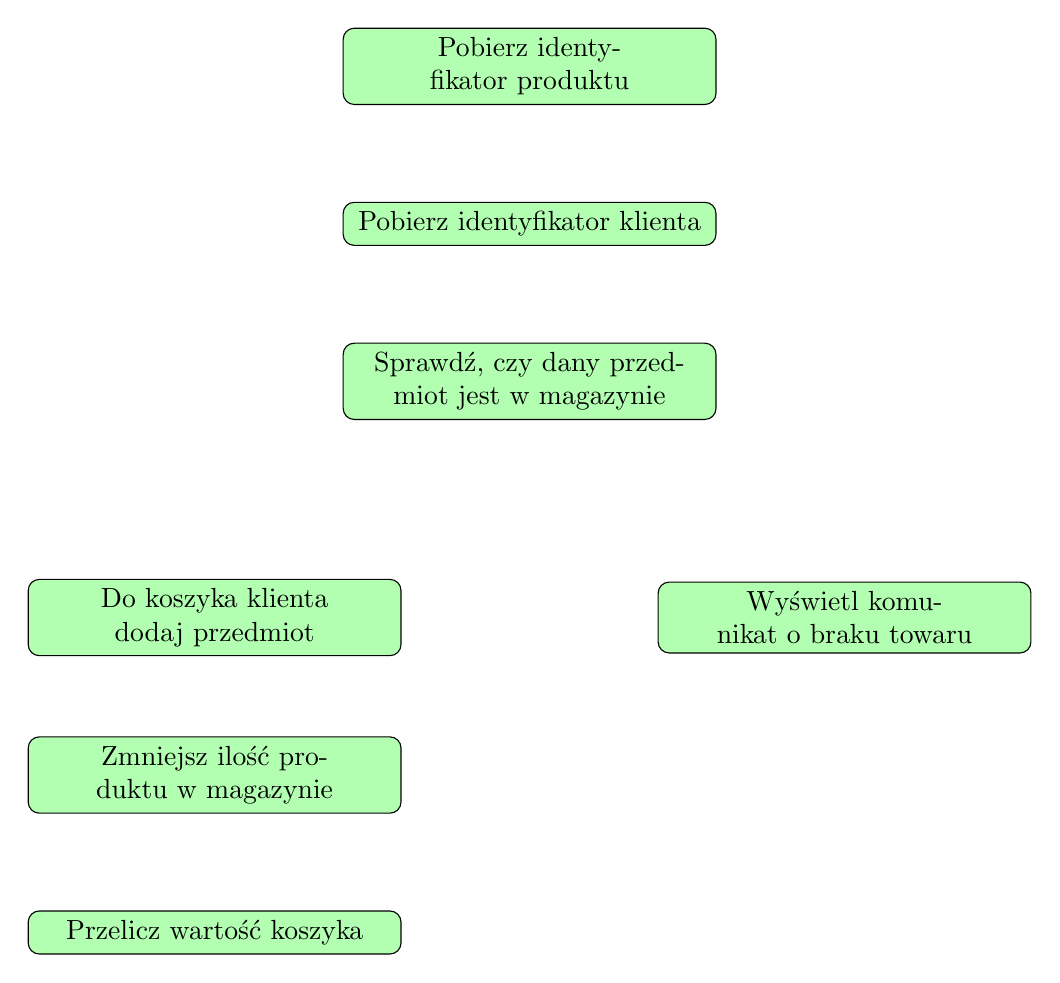
\begin{tikzpicture}
        \umlstateinitial[name=begin]
        \node[singlestate] at (4,0) (getId){Pobierz identyfikator produktu};
        \node[singlestate] at (4,-2) (getUser){Pobierz identyfikator klienta};
        \node[singlestate] at (4,-4) (checkAmount){Sprawdź, czy dany przedmiot jest w magazynie};
        \umlstatedecision[x=4,y=-7,name=check]
        \node[singlestate] at (0,-7) (success){Do koszyka klienta dodaj przedmiot};
        \node[singlestate] at (8,-7) (error){Wyświetl komunikat o braku towaru};
        \node[singlestate] at (0,-9) (removeFromStock){Zmniejsz ilość produktu w magazynie};
        \node[singlestate] at (0,-11) (countValue){Przelicz wartość koszyka};
        \umlstateexit[x=0,y=-12.5,name=exit1]
        \umlstateexit[x=8,y=-8.5,name=exit2]
        
        \umltrans{begin}{getId}
        \umltrans{getId}{getUser}
        \umltrans{getUser}{checkAmount}
        \umltrans{checkAmount}{check}
        \umltrans[arg=Jest, pos=0.5]{check}{success}
        \umltrans[arg=Brak, pos=0.3]{check}{error}
        \umltrans{success}{removeFromStock}
        \umltrans{removeFromStock}{countValue}
        \umltrans{countValue}{exit1}
        \umltrans{error}{exit2}
        
    \end{tikzpicture}}
\end{figure}

\subsection{Diagram klas}
\begin{figure}[H]
    \centering
    \includegraphics[scale=.7]{Pics/classDiagram.png}
\end{figure}

\newpage
\section{Harmonogram prac}

\begin{figure}[H]
    \centering
    \begin{turn}{90}
\begin{ganttchart}[
    % today=53,
    % today rule/.style= {thick},
    x unit=0.25cm,
    y unit title=0.7cm,
    y unit chart=0.7cm,
    progress label text={},
    bar height=0.7,
    group label font=\bfseries,
    milestone label font=\tiny\itshape,
    title height=1,
    bar/.style={draw=black, fill=gray!50},
    bar incomplete/.style={draw=black, fill=white},
    vgrid, hgrid]{1}{56}
    \gantttitle{2019}{56} \\
    % \gantttitle{2018}{24} \\
    \gantttitle{Październik}{17}
    \gantttitle{Listopad}{30}2
    \gantttitle{Grudzień}{9} \\
    % \gantttitle{January}{4}
    % \gantttitle{February}{4}
    % \gantttitle{March}{4}
    % \gantttitle{April}{4} 
    % \gantttitle{May}{4}
    % \gantttitle{June}{4} \\
    \ganttgroup{Projektowanie}{1}{21} \\
    \ganttbar[progress=100]{Cel i zakres}{1}{14} \\
    \ganttbar[progress=100]{Analiza SWOT}{8}{21} \\
    \ganttbar[progress=100]{Diagramy UML}{12}{21} \\
    \ganttbar[progress=100]{Kosztorys}{15}{21} \\
    \ganttgroup{Implementacja}{15}{50} \\
    \ganttbar[progress=100]{Stworzenie projektu}{15}{21} \\
    \ganttbar[progress=100]{Stworzenie bazy danych}{15}{28} \\
    \ganttbar[progress=100]{Połączenie z bazą}{22}{28} \\
    \ganttbar[progress=100]{Stworzenie kontrolerów}{22}{50} \\
    \ganttbar[progress=100]{Stworzenie front-endu}{29}{50} \\
    \ganttgroup{Wdrożenie}{51}{56} \\
    \ganttbar[progress=100]{Prezentacja projektu}{51}{56} \\
    % \ganttbar[progress=0]{}{29}{29} % <-- empty label
    % \ganttmilestone{Task 11}{35}
    
    % \ganttlink{elem6}{elem9}
    % \ganttlink{elem6}{elem8}
\end{ganttchart}
\end{turn}
% \caption{Harmonogram zadań}

\end{figure}

\newpage
\section{Przewodnik po witrynie}

\subsection{Rejestracja w serwisie}
Pierwszym krokiem będzie utworzenie konta użytkownika. W tym celu przechodzimy na stronę rejestracji (podstrona \textit{/registration}), gdzie ukaże nam się formularz widoczny poniżej. Aby zarejestrować nowego użytkownika należy podać:
\begin{enumerate}
    \item Imię
    \item Nazwisko
    \item Adres e-mail (dla każdego konta unikalny)
    \item Hasło do konta
\end{enumerate}
\begin{figure}[H]
    \centering
    \includegraphics[scale=.47]{Pics/registration.png}
    \caption{Ekran rejestracji}
    \label{pic:registration}
\end{figure}
W celu sfinalizowania procesu należy kliknąć przycisk (5). Pojawi się odpowiedni komunikat, w zależności od powodzenia operacji. Po pomyślnej rejestracji możemy przejść do następnego kroku klikając w link (6).

\subsection{Logowanie do konta}
Aby móc dokonywać zakupów, musimy wcześniej zalogować się do uprzednio utworzonego konta. W tym celu musimy uzupełnić wymagane pola:
\begin{enumerate}
    \item Adres e-mail podany przy rejestracji
    \item Hasło do konta, również podane podczas rejestracji
\end{enumerate}
\begin{figure}[H]
    \centering
    \includegraphics[scale=.5]{Pics/login.png}
    \caption{Ekran logowania}
    \label{pic:login}
\end{figure}
Następnie należy kliknąć przycisk (3). Jeśli jeszcze nie założyliśmy konta, możemy bardzo łatwo przenieść się na stronę z rejestracją, wystarczy kliknąć odnośnik (4).

\subsection{Strona główna}
Na stronie głównej wyświetlane są wszystkie towary dostępne w sklepie. W tym miejscu mamy dostęp do wszystkich podstron witryny. Możemy:
\begin{enumerate}
    \item Przejść do strony konkretnego produktu
    \item Zalogować się lub założyć nowe konto
    \item W przypadku konta z uprawnieniami administratora wyświetlić panel zarządzania zawartością sklepu
    \item Przejrzeć zawartość koszyka
\end{enumerate}
Design strony jest responsywny, oznacza to, że dopasowuje się do ekranu urządzenia (przykładowo, na smartfonie lub tablecie wygląd sklepu będzie się nieznacznie różnił od wersji przygotowanej na komputery PC, tak aby maksymalnie zwiększyć wygodę obsługi na mniejszym wyświetlaczu). W wersji mobilnej odnośniki z nagłówka strony są schowane w menu po lewej stronie (2).
\begin{figure}[H]
    \centering
    \includegraphics[scale=.2]{Pics/mobileMainPage.png}
    \caption{Strona główna serwisu w wersji mobilnej}
    \label{pic:mobileMainPage}
\end{figure}
\begin{figure}[H]
    \centering
    \includegraphics[width=14cm]{Pics/mainPage.png}
    \caption{Strona główna serwisu w standardowej wersji}
    \label{pic:mainPage}
\end{figure}

\subsection{Strona produktu}
Po wybraniu linku (1) na poprzedniej stronie ukaże nam się strona danego produktu. Tutaj mamy możliwość zobaczyć szczegóły towaru:
\begin{enumerate}
    \item Zdjęcia w pełnym rozmiarze
    \item Cenę netto
    \item Ilość w magazynie
    \item Opis
\end{enumerate}
Przycisk (5) służy do dodawania przedmiotu do naszego koszyka. Po jego kliknięciu, jeśli nie jesteśmy zalogowani, zostaniemy o to poproszeni. Jeśli towar jest dostępny (w magazynie znajduje się więcej niż 1 sztuka) to zostanie on przekazany do koszyka użytkownika, a na stronie pojawi się odpowiedni komunikat potwierdzający. W przeciwnym wypadku wyświetlony komunikat będzie zawierał informację o problemie.\\
Dodatkowo, pole (6) zawiera proponowane produkty, które mogą zainteresować klientów. 
\begin{figure}[H]
    \centering
    \includegraphics[width=14cm]{Pics/product1.png}
    \caption{Strona produktu}
    \label{pic:productPage1}
\end{figure}
\begin{figure}[H]
    \centering
    \includegraphics[scale=.2]{Pics/product2.png}
    \caption{Strona produktu w wersji mobilnej}
    \label{pic:productPage2}
\end{figure}

\subsection{Koszyk}
W dowolnej chwili można sprawdzić zawartość koszyka. Aby to zrobić należy kliknąć w ikonkę wózka sklepowego umieszczoną po prawej stronie nagłówka. Wyświetli się tam lista wybranych przedmiotów wraz z podsumowaniem zamówienia (doliczenie do sumy podatku i kosztów dostawy). Jeśli koszyk nie będzie zawierał żadnych przedmiotów, zostanie wyświetlony odpowiedni komunikat. 
\begin{figure}[H]
    \centering
    \includegraphics[width=13cm]{Pics/cart2.png}
    \caption{Pusty koszyk}
    \label{pic:cartEmpty}
\end{figure}
\begin{figure}[H]
    \centering
    \includegraphics[width=13cm]{Pics/cart3.png}
    \caption{Koszyk z zawartością}
    \label{pic:cartFull}
\end{figure}

\subsection{Panel administratora}
Wstęp do tej podstrony mają tylko użytkownicy z przyznanymi uprawnieniami administratora. Tutaj można zarządzać zawartością bazy danych, a konkretnie:
\begin{itemize}
    \item wyświetlać listę użytkowników i ich dane
    \item wyświetlać listę produktów
    \item dodawać nowe produkty i zarządzać istniejącymi
    \item przeglądać i zarządzać kategoriami towarów
    \item wyświetlać bieżące koszyki klientów
    \item wyświetlać listę złożonych zamówień
\end{itemize}
\begin{figure}[H]
    \centering
    \includegraphics[width=15cm]{Pics/adminPanel1.png}
    \caption{Panel zarządzania zawartością sklepu}
    \label{pic:adminPanel1}
\end{figure}
\begin{figure}[H]
    \centering
    \includegraphics[width=15cm]{Pics/adminPanel2.png}
    \caption{Lista złożonych zamówień}
    \label{pic:adminPanel2}
\end{figure}
\begin{figure}[H]
    \centering
    \includegraphics[width=15cm]{Pics/adminPanel3.png}
    \caption{Lista użytkowników systemu}
    \label{pic:adminPanel3}
\end{figure}

\subsection{Obsługa błędów}
Jak wiadomo, błędy się zdarzają, dlatego na wypadek różnych sytuacji, gdzie niemożliwe będzie wyświetlenie strony (np. klient spróbuje wyświetlić produkt, który zostanie w tym momencie usunięty, lub będzie chciał podmienić numer id produktu w pasku adresu na nieistniejący) przygotowana została strona obsługująca błąd HTTP 404. Jest to prosty szablon z czytelną informacją, która powiadomi użytkownika, że żądana strona nie istnieje.
\begin{figure}[H]
    \centering
    \includegraphics[width=15cm]{Pics/404.png}
    \caption{Błąd HTTP 404}
    \label{pic:404}
\end{figure}

\subsection{Polityka prywatności i informacja o ciasteczkach (ang. cookies)}
Każda strona przechowująca dane osobowe klienta lub dane cookies, musi go o tym poinformować. Nasz serwis zawiera odpowiednią stronę, w której jest dokładnie opisane jakie dane są przechowywane na serwerze. Do wygenerowania powyższego oświadczenia posłużyła nam strona Privacy Policy Generator \hyperlink{https://www.privacypolicygenerator.info}{(link tutaj)}.
\begin{figure}[H]
    \centering
    \includegraphics[width=13cm]{Pics/privacy.png}
    \caption{Polityka prywatności firmy}
    \label{pic:privacy}
\end{figure}
\begin{figure}[H]
    \centering
    \includegraphics[width=15cm]{Pics/cookies.png}
    \caption{Okienko z informacją o przechowywaniu ,,ciasteczek''}
    \label{pic:cookies}
\end{figure}

\newpage
\section{Wdrożenie aplikacji}
Aplikacja powinna zostać wdrożona przy użyciu pliku jar. Aby spakować aplikację do jednego (grubego) pliku jar, należy uruchomić polecenie \mintinline{java}{mvn package} w katalogu projektu. Spowoduje to spakowanie aplikacji do pliku wykonywalnego jar wraz ze wszystkimi jej zależnościami (w tym osadzony kontener serwletu). Aby uruchomić plik jar, należy użyć następującej standardowej komendy JVM \mintinline{java}{java -jar <nazwa_pliku_jar>.jar}.\\

Jedną z możliwości wdrożenia jest wykorzystanie Heroku. Jest to platforma chmurowa stworzona w modelu PaaS (Platform as a Service) obsługująca kilka języków programowania~\cite{heroku}. Jednym z nich jest właśnie Java. Wdrożenie aplikacji jest bardzo proste i polega na wykonaniu tylko kilku komend z poziomu CLI Heroku. Łączy się on z GitHubem i automatycznie buduje aplikację z gałęzi master, więc można go wykorzystać jako jedno z narzędzi do CI/CD.

\newpage
\section{Wnioski}
Tworzenie aplikacji webowych z dostępem do bazy danych nie jest łatwe. Dlatego nieustannie rozwijane są produkty, które pomagają uprościć niektóre etapy. Kolejną zaletą takiego rozwiązania jest usystematyzowanie pewnych elementów aplikacji, dzięki czemu zespół rozwijający system może bez problemów ,,odnaleźć się'' w kodzie pisanym przez kogoś innego. To z kolei przekłada się na szybszą pracę nad projektem, który będzie mógł przynosić zyski zleceniodawcy dużo wcześniej. \\\\
Niestety, nie udało nam się zaimplementować funkcji związanych z finalizacją zamówień i wyszukiwarką produktów na stronie głównej. Są to procesy mocno skomplikowane i przez to czasochłonne, a nasze priorytety były skupione na pozostałych funkcjach.\\\\
\large{Link do repozytorium: \rotatebox[origin=c]{270}{$\Rsh$}}\\ \hyperlink{https://github.com/jastka4/idb-skate-shop}{https://github.com/jastka4/idb-skate-shop}

\newpage
\bibliographystyle{unsrt}
\bibliography{references}

\end{document}
